\chapter{Машинное обучение}
\label{ch:ml}

\section{Градиентный спуск}
Пусть мы имеем функцию $z = sin(x)sin(y)$ (см. \autoref{ml:descent:sin}) и нам надо, находясь в какой-либо точке, добраться до наивысшей из этой точки, иначе говоря, найти локальный максимум функции $z$. Для быстрейшего достижения локального максимума целесообразно двигаться в направлении наискорейшего возрастания функции $z$, иначе: вдоль градиента.

\IfNotDraft
{
\begin{figure}[htb]
  \centering
  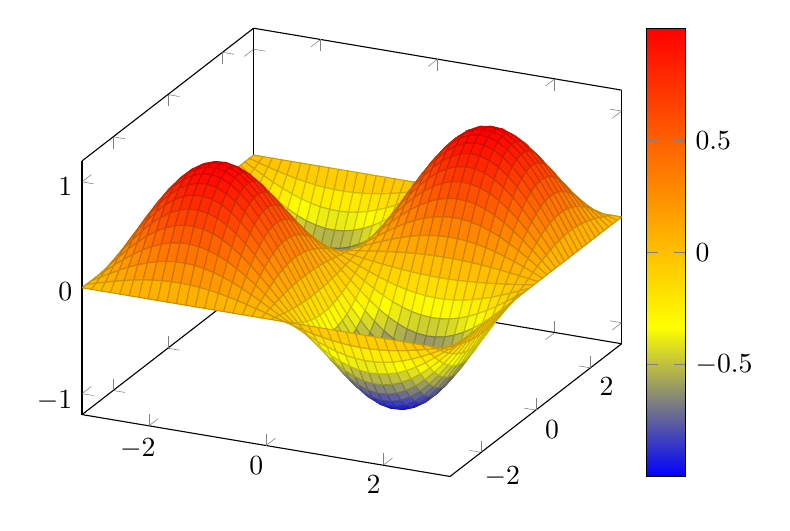
\begin{tikzpicture}
    \begin{axis}[colorbar]
      \addplot3[
        surf,
        domain=-pi:pi,
        samples=40] {
          sin(deg(x))*sin(deg(y))
        };
    \end{axis}
  \end{tikzpicture}
  \caption{График функции $z = sin(x)sin(y)$}
  \label{ml:descent:sin}
\end{figure}
}

В этом и состоит смысл алгоритма \emph{градиентного спуска}: шагаем вдоль градиента до тех пор, пока не остановимся (ну, или почти). Пусть мы находимся в некоторой точке $\theta$, тогда обновление её координат происходит следующим образом:
\[
\theta_j = \theta_j - \alpha\frac{\partial}{\partial\theta_j}J(\theta),
\]
где $J(\theta)$ — матрица Якоби. По приведённой формуле можно найти локальные \emph{минимум} функции. Для нахождения же \emph{максимума} следует использовать в формуле плюс вместо минуса.

\begin{pylst}{Реализация градиентного спуска}{}
import operator

from numpy import *

def sinsin_gradient(vec):
    x, y = vec
    return array([cos(x) * sin(y),
                  sin(x) * cos(y)])

def gdescent(initial, gradient_fn, step_fn=operator.sub,
             maxiter=1000, eps=0.01, precision=0.00001):

    x = initial
    for i in range(maxiter):
        old_x = x.copy()
        x = step_fn(old_x, eps * gradient_fn(x))

        if sum((x - old_x) ** 2) < precision:
            break

    return x
\end{pylst}

Ниже представлены промежуточные результаты алгоритма для начальной точки $[2; -1]$.
\IfNotDraft
{
\begin{figure}[htb]
  \centering
  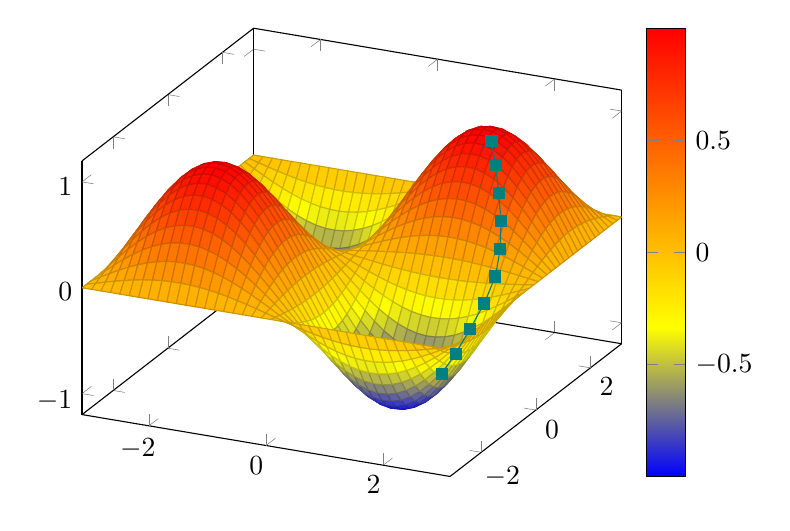
\begin{tikzpicture}
    \begin{axis}[colorbar]
      \addplot3[
        surf,
        domain=-pi:pi,
        samples=40] {
          sin(deg(x))*sin(deg(y))
        };

     \addplot3+[teal,mark options=teal] coordinates {
       (2.00,-1.00,-0.76)
       (2.14,-0.79,-0.60)
       (2.28,-0.56,-0.40)
       (2.40,-0.30,-0.20)
       (2.45,0.00,0.00)
       (2.40,0.29,0.20)
       (2.29,0.55,0.40)
       (2.14,0.79,0.60)
       (1.97,1.04,0.80)
       (1.77,1.32,0.95)
     };
    \end{axis}
  \end{tikzpicture}
\end{figure}
}

\subsection{Применение к обучению}
Допустим, у нас есть табличные данные о площади квартир, количестве комнат в каждой из них и их стоимости.
\begin{table}[h!]
  \centering
  \begin{tabular}{ccc}
    \toprule
    \textbf{Жилая площадь ($\text{м}^2$)} & \textbf{Кол-во комнат} & \textbf{Стоимость ($1000\$$)} \\
    \midrule
    120 & 4 & 157 \\
    90  & 3 & 120 \\
    …   & … & …   \\
    \bottomrule
  \end{tabular}
\end{table}

Перед нами стоит задача аппроксимировать табличные данные функцией какого-либо вида. В данном случае выбор линейной функции — годится.
\[
h_\theta(x) = \theta_0 + \theta_1 x_1 + \theta_2 x_2,
\]
где $\theta_i$ — параметры (или веса), а $x_0 = 1$. Тогда
\[
h(x) = \sum_{i = 0}^n \theta_i x_i = \theta^T x.
\]

Теперь нам надо как-то получить конкретные значения параметров $\theta_i$. Попытаемся приблизить $h(x)$ к тестовым данным как можно ближе. Для этого введём \emph{функцию стоимости}:
\[
J(\theta) = \frac{1}{2} \sum_{i = 1}^m (h_\theta(x^{(i)}) - y^{(i)})^2.
\]

Очевидно, для достижения поставленной цели эту функцию нужно минимизировать. Производная этой функции по параматру $\theta_j$ равна:
\begin{align*}
\frac{\partial}{\partial \theta_j} J(\theta) &= \frac{\partial}{\partial \theta_j} \frac{1}{2} (h_\theta(x) - y)^2 \\
                                             &= 2 \cdot \frac{1}{2} (h_\theta(x) - y) \frac{\partial}{\partial \theta_j} (h_\theta(x) - y) \\
                                             &= (h_\theta(x) - y) \cdot \frac{\partial}{\partial \theta_j} \left( \sum_{i = 0}^n \theta_i x_i - y \right) \\
                                             &= (h_\theta(x) - y) x_j.
\end{align*}

Поэтому правило обновления параметров получается следующим, используя метод градиентного спуска:
\[
\theta_j = \theta_j - \alpha (h_\theta(x)^{(i)} - y^{(i)}) x_j^{(i)}.
\]

Вышеприведённая формула — для случае, когда тестовый набор данных состоит всего лишь из одной записи. Если же записей $m$, то
\[
\theta_j = \theta_j - \alpha \sum_{i = 1}^m (h_\theta(x)^{(i)} - y^{(i)}) x_j^{(i)}.
\]

В результате мы получим \emph{глобальный} минимум, так как функция стоимости имеет только один минимум, а максимума не имеет.

\subsubsection{Пример}

Мы имеем небольшие данные о цене квартир и их площадях. Попытаемся найти параметры $\theta_0$ и $\theta_1$.
\begin{pylst}{}{}
def lg_gradient(p):
    def fn(x):
        return p[0] + p[1] * x

    result = array([0 for _ in range(len(p))])
    for x, y in samples:
        result += (fn(x) - y) * array([1.0, x])

    return result

>>> gdescent(array([20.0, 0.1]), lg_gradient, eps=0.00000001)
[ 19.99998493   0.06248649]
\end{pylst}

Следовательно, $\theta_0 = 19.999$ и $\theta_1 = 0.0624$. Функция $price = \theta_0 + \theta_1 square$ проиллюстрирована на \autoref{ml:descent:lms}.

\begin{figure}[htb]
  \centering
  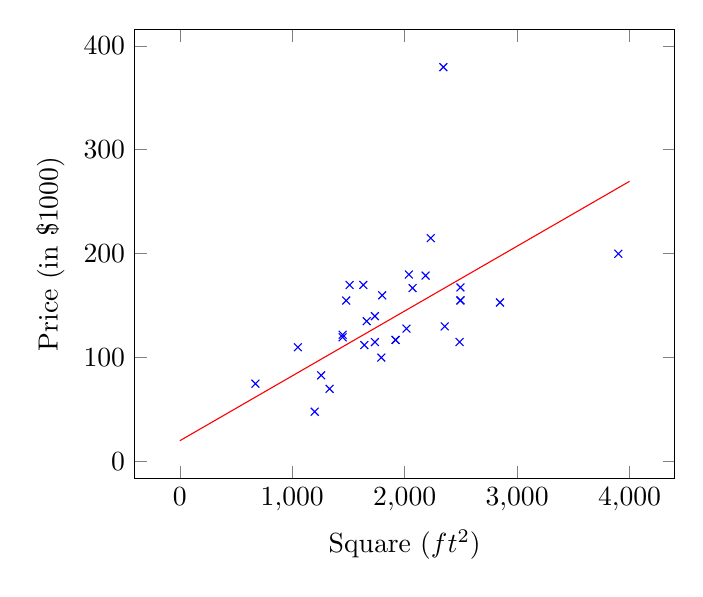
\begin{tikzpicture}
    \begin{axis}[
      xlabel=Square ($ft^2$),
      ylabel=Price (in \$1000)]
     \addplot+[only marks,mark=x] coordinates {
       (1641,112.0)
       (2232,214.9)
       (1050,109.9)
       (2496,155)
       (1919,117)
       (672,74.9)
       (1448,119.5)
       (1448,122)
       (1662,135)
       (1800,159.9)
       (3900,199.9)
       (1200,47.9)
       (2016,127.9)
       (2496,167.5)
       (1735,114.9)
       (2848,153)
       (1257,82.9)
       (1480,154.9)
       (2496,155)
       (1332,69.9)
       (1792,100)
       (2037,179.9)
       (2488,115)
       (2356,130)
       (1919,117)
       (2186,178.9)
       (2070,166.9)
       (1632,169.9)
       (1735,139.9)
       (1510,169.9)
       (2344,379.5)
     };

     \addplot+[no marks,domain=0:4000]{19.999 + 0.0624*x};
    \end{axis}
  \end{tikzpicture}
  \caption{Обучающая выборка и аппроксимированая функция.}
  \label{ml:descent:lms}
\end{figure}

\section{Кластеризация}
\emph{Кластеризация} — метод обнаружения групп (кластеров) связанных между собой объектов. Кластеризация — пример обучения без учителя.

\subsection{Алгоритм $k$ средних}
Пусть имеется тестовый набор данных $x^{(1)}, \dots, x^{(m)}$, где $x^{(i)} \in \mathbb{R}^n$. Наша цель — выделить $k$ групп из этого набора, где $k$ — предварительно задано. Тогда алгоритм $k$ средних следующий:
\begin{enumerate}
  \item Выбрать случайно центроиды кластеров $\mu^{(1)}, \dots, \mu^{(k)}$, где $\mu^{(i)} \in \mathbb{R}^n$.
  \item Повторять до сходимости (до тех пор, пока центры кластеров не станут постоянными):
    \begin{enumerate}
      \item Для каждого $i$, присвоить \[ c^{(i)} = \operatorname*{arg\,min}_j \| x^{(i)} - \mu_j \|^2. \]
      \item Для каждого $j$, присвоить \[ \mu_j = \frac{\sum_{i = 1}^{m}{1\{ c^{(i)} = j \} x^{(i)}}}{\sum_{i = 1}^{m}{1\{ c^{(i)} = j \}}}. \]
    \end{enumerate}
\end{enumerate}

Этот же алгоритм на пальцах:
\begin{enumerate}
  \item Проинициализировать.
  \item Классифицировать точки по ближайшему к ним центру кластера.
  \item Перевычислить каждый из центров.
  \item Если центры изменились, то повторить с пункта $2$.
\end{enumerate}

Этот алгоритм имеет некоторые недостатки:
\begin{itemize}
  \item Неопределенность с методом выбора начальных центров кластеров.
  \item Количество кластеров надо знать заранее.
  \item Вычислительно сложен.
  \item Качество результата зависит от разбиения, которое в свою очередь завист от выбора начальных центров.
\end{itemize}

\subsection{Метрики}
Нужно уметь вычислять похожесть (расстояние, удалённость) конкретного элемента из набора данных на какой-либо центр. Мы рассмотрим две метрики, используемых в алгоритме $k$ средних. Одна из них — евклидова, другая — коэффициент корреляции Пирсона.

\subsubsection{Евклидова метрика}
Евклидова метрика $d(p, q)$ — это расстояние между двумя точками $p$ и $q$. Пусть $p = (p_1, \dots, p_n)$ и $q = (q_1, \dots, q_n)$, тогда:
\[
d(p, q) = \sqrt{\sum_{k = 1}^n (p_k - q_k)^2}.
\]

В следующей реализации мы возвращаем обратное значение расстояния, так как нужно, чтобы значение для похожих элементов было больше, чем для непохожих. Добавляем же мы единицу в знаменателе для того, чтобы избежать деления на ноль. Квадратный корень не извлекается, так как не важны конкретные значения метрики, а важно то, чтобы соблюдалось правило, что для похожих элементов метрика даёт больший результат, чем для менее похожих.
\begin{pylst}{}{}
from math import sqrt

def sim_distance(vec1, vec2):
    assert len(vec1) == len(vec2)
    sum_of_squares = sum(pow(v1 - v2, 2)
                         for v1, v2 in zip(vec1, vec2))

    return 1 / (1 + sum_of_squares)
\end{pylst}

\subsubsection{Коэффициент корреляции Пирсона}
\emph{Коэффициент корреляции Пирсона} — это мера корреляции двух случайных величин \(X\) и \(Y\). Он принимает значения от \(-1\) до \(+1\), включая концы. Коэффициент определён следующим образом:
\[
\rho_{X, Y} = \frac{cov(X, Y)}{\sigma_X \sigma_Y} = \frac{E[(X - \mu_X)(Y - \mu_Y)]}{\sigma_X \sigma_Y},
\]
где \(cov\) — ковариация, \(E\) — оператор математического ожидания, а \(\mu_X\) и \(\mu_Y\) — среднеквадратичные отклонения.

Этот же коэффициент, но определённый для конкретных выборок и подсчитанный, используя оценки ковариации и среднеквадратичных отклонений:
\begin{align*}
r &= \frac{\frac{1}{n - 1} \sum_{i = 1}^n (X_i - \bar{X})(Y_i - \bar{Y})}{\sqrt{\frac{1}{n - 1} \sum_{i = 1}^n (X_i - \bar{X})^2} \sqrt{\frac{1}{n - 1} \sum_{i = 1}^n (Y_i - \bar{Y})^2}} = \\
  &= \frac{\sum_{i = 1}^n (X_i - \bar{X})(Y_i - \bar{Y})}{\sqrt{\sum_{i = 1}^n (X_i - \bar{X})^2} \sqrt{\sum_{i = 1}^n (Y_i - \bar{Y})^2}},
\end{align*}
где \(\bar{X}\) и \(\bar{Y}\) — средние значения выборок. Они равны \(\frac{1}{n} \sum_{i = 1}^n X_i\) и \(\frac{1}{n} \sum_{i = 1}^n Y_i\), соответственно.

Те же яйца, вид сбоку:
\[
r = \frac{1}{n - 1} \sum_{i = 1}^n \left( \frac{X_i - \bar{X}}{s_X} \right) \left( \frac{Y_i - \bar{Y}}{s_Y} \right).
\]

Можно вывести представить эту формулу так, что алгоритмическая сложность вычисления будет меньше. Учитывая, что
\[
E[(X - \mu_X)(Y - \mu_Y)] = E(XY) - \mu_X \mu_Y,
\]
тогда
\begin{align*}
\rho_{X, Y} &= \frac{E[(X - \mu_X)(Y - \mu_Y)]}{\sqrt{(E[(X - \mu_X)^2])} \sqrt{(E[(Y - \mu_Y)^2])}} = \\
  &= \frac{E(XY) - \mu_X \mu_Y}{\sqrt{(E[X^2] - \mu_X^2)} \sqrt{(E[Y^2] - \mu_Y^2)}}. \\
r &= \frac{\frac{1}{n} \sum_{i = 1}^n{X_i Y_i} - \frac{1}{n^2} \sum_{i = 1}^n{X_i} \sum_{i = 1}^n{Y_i}}{\sqrt{\frac{1}{n}\sum_{i = 1}^n{X_i^2} - (\frac{1}{n}\sum_{i = 1}^n{X_i})^2} \sqrt{\frac{1}{n}\sum_{i = 1}^n{Y_i^2} - (\frac{1}{n}\sum_{i = 1}^n{Y_i})^2}} = \\
  &= \frac{\sum_{i = 1}^n{X_i Y_i} - \frac{\sum_{i = 1}^n{X_i} \sum_{i = 1}^n{Y_i}}{n}}{\sqrt{\sum_{i = 1}^n{X_i^2} - \frac{\left(\sum_{i = 1}^n{X_i}\right)^2}{n}} \sqrt{\sum_{i = 1}^n{Y_i^2} - \frac{\left(\sum_{i = 1}^n{Y_i}\right)^2}{n}}}.
\end{align*}

Предположим, что два критика выставили некоторые оценки различным исполнениям чаконны из партиты №2 для скрипки соло И.С. Баха. Значение коэффициента \(-1\) означает, что критики выставили полностью противоположные оценки: где один оценил исполнение высоко, другой оценил низко, и наоборот. Можно сказать, что между их оценками есть зависимость.

Значение \(1\) означает, что критики оценивают исполнения одинаково, но каждый по своей шкале. Так если было три исполнения, и первый критик выставил оценки \([1, 2, 3]\), а второй критик выставил — \([1, 3, 5]\), то всё-равно коэффициент Пирсона будет равен единице.

Значение \(0\) означает, что зависимости в выставлении оценок у критиков нет.
\begin{table}[h!]
  \caption{Интерпретация значений}
  \begin{center}
    \begin{tabular}{lll}
      \toprule
      \textbf{Корреляция} & \textbf{Отрицательный} & \textbf{Положительный} \\
      \midrule
      Нет     & \texttt{[-0.09; 0.0]} & \texttt{[0.0; 0.09]} \\
      Малая   & \texttt{[-0.3; -0.1]} & \texttt{[0.1; 0.3]} \\
      Средняя & \texttt{[-0.5; -0.3]} & \texttt{[0.3; 0.5]} \\
      Большая & \texttt{[-1.0; -0.5]} & \texttt{[0.5; 1.0]} \\
      \bottomrule
    \end{tabular}
  \end{center}
\end{table}

\begin{pylst}{Функция вычисления коэффициента Пирсона}{}
def sim_pearson(vec1, vec2):
    assert len(vec1) == len(vec2)

    n = len(vec1)
    if n == 0:
        return 0

    sum1, sum2 = sum(vec1), sum(vec2)
    sum1_of_squares = sum(pow(v, 2) for v in vec1)
    sum2_of_squares = sum(pow(v, 2) for v in vec2)
    sum_of_products = sum(v1 * v2 for v1, v2 in zip(vec1, vec2))

    num = sum_of_products - (sum1 * sum2 / n)
    den = sqrt((sum1_of_squares - pow(sum1, 2) / n) *
               (sum2_of_squares - pow(sum2, 2) / n))

    if den == 0:
        return 0

    r = num / den
    return r
\end{pylst}

\subsection{Реализация алгоритма $k$ средних}

\begin{pylst}{}{}
from numpy import *
from metrics import sim_distance

def kmeans(data, distance=sim_distance, k=3, iternum=100, err=0.0005):
    vecnum, veclen = data.shape
    minima = data.min(axis=0)
    maxima = data.max(axis=0)

    centroids = random.rand(k, veclen) * (maxima - minima) + minima
    clusters = None

    for t in range(iternum):
        distances = zeros(shape=(k, vecnum))
        for i in range(k):
            distances[i] = sum((data - centroids[i,:])**2, axis=1)

        clusters = distances.argmin(axis=0)
        clusters.shape = (vecnum, 1)

        old_centroids = centroids.copy()
        for i in range(k):
            cluster = where(clusters == i, 1, 0)
            if sum(cluster) > 0:
                centroids[i,:] = sum(data * cluster, axis=0) / sum(cluster)

        if abs(sum(centroids - old_centroids)) < err:
            break

    return centroids, clusters
\end{pylst}

\subsection{Пример кластеризации: ирисы Фишера}
Набор данных состоит из записей, содержащих данные о длине и ширине чашелистика, длины и ширины лепестка и, собственно, сорта ириса.
\begin{plainlst}{}{}
5.1,3.5,1.4,0.2,setosa
...
7.0,3.2,4.7,1.4,versicolor
...
6.3,3.3,6.0,2.5,virginica
...
\end{plainlst}

На \autoref{ml:fig:iris-dataset-visualization} представлены графики, построенные по этому набору данных.

\IfNotDraft
{
\begin{figure}[tb]
  \begin{center}
    \leavevmode
    \includegraphics[width=0.8\textwidth]{images/ml/iris-flower-dataset}
  \end{center}
  \caption{Визуализация набора данных ``Ирисы Фишера''. setosa — красный, versicolor — зелёный, virginica — синий.}
  \label{ml:fig:iris-dataset-visualization}
\end{figure}
}

На \autoref{ml:fig:iris-dataset-kmeans} иллюстрирован возможный результат алгоритма $k$ средних.

\IfNotDraft
{
\begin{figure}[tb]
  \begin{center}
    \leavevmode
    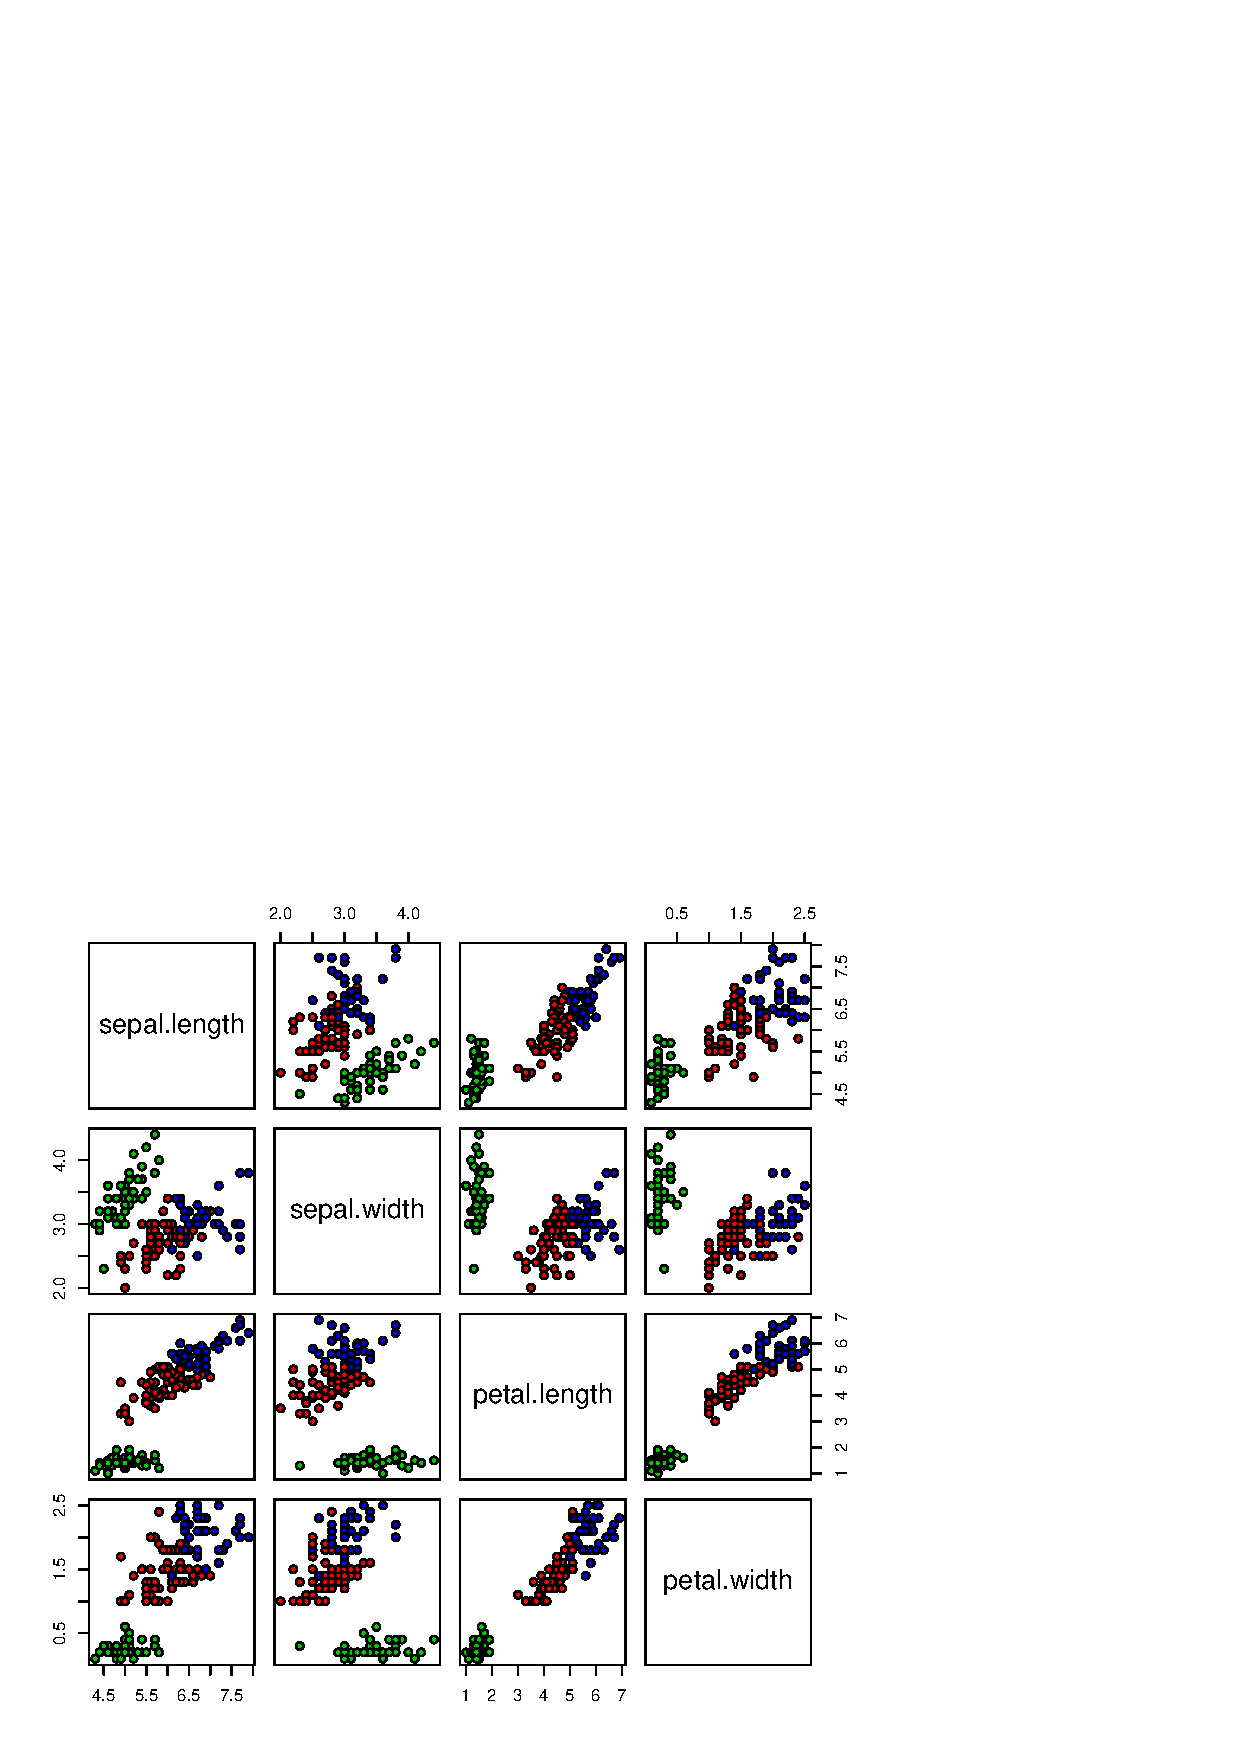
\includegraphics[width=0.8\textwidth]{images/ml/iris-flower-kmeans}
  \end{center}
  \caption{Визуализация клустеризации набора данных ``Ирисы Фишера''.}
  \label{ml:fig:iris-dataset-kmeans}
\end{figure}
}

\section{Классификация}
\emph{Классификация} объекта — это указание класса для данного объекта. Например, по значениям длин и ширин чашелистника и лепестка цветка ириса нужно определить его вид.

\subsection{Метод $k$ ближайших соседей}
Суть \emph{метода $k$ ближайших соседей} (англ. k-nearest neighbor algorithm) состоит в том, что объекту присваивается тот класс, который является наиболее распространённым среди его $k$ соседей. Из этого следует, что нужно иметь набор данных с заранее известными классами объектов.

Для определения близости, как правило, используется евклидова метрика.

Предельно наивная реализация данного алгоритма — предельно очевидна. Она же — приведена ниже:
\begin{pylst}{Наивная реализация kNN}{}
def knn(item, dataset):
    klass = None
    nearest = None

    for row in dataset:
        next = metrics.sim_distance(item, row["features"])

        if nearest is None:
            nearest =  next
        elif next > nearest:
            klass = row["class"]
            nearest = next

    return klass
\end{pylst}

Пример запуска для набора данных ``Ирисы Фишера'':
\begin{pylst}{}{}
>>> knn([4.5, 3.8, 1.2, 0.4], dataset)
"setosa"
\end{pylst}

\subsection{kd деревья}
\emph{kd дерево} (англ. k-dimensional tree) — структура данных, используемая для разбития $k$-размерного пространства на подпространства по некоторым заданных точкам.

kd дерево — это бинарное дерево, в котором каждый узел содержит точку пространства размерности $k$. Каждый внутренний узел представляет собой точку, через которую проходит гиперплоскость, разбивающая пространство на две части. При этом точки из левого поддерева находятся по одну сторону от этой гиперплоскости, точки же правого поддерева — по другую.

Направление гиперплоскостей выбирается следующим образом: выбирается какая-либо ось, и гиперплоскость строится перпендикулярно к этой оси. Например, допустим выбрана ось $x$, тогда все точки текущего поддерева, у которых координата по оси $x$ меньше, будут находится по одну сторону от гиперплоскости, проведённой через точку $(x_{concrete}, 0, \dots)$; оставшиеся же точки — по другую сторону. При этом первые — будут в левом поддереве, вторые же — в правом.

\subsubsection{Построение kd дерева}
Так как способов выбирать следующую ось, перпендикулярно которой строится следующая гиперплоскость, — много, то и построений может быть — много. Каноническим способом является:
\begin{itemize}
  \item Циклически и последовательно выбирать следующую ось по порядку, начиная с оси $x$, для каждого следующего уровня дерева.
  \item Элементом текущего узла является точка, которая является медианой точек текущего поддерева.
\end{itemize}

Посмотрим дерево для точек $(2; 3), (5; 4), (9; 6), (4; 7), (8; 1), (7; 2)$. Оно будет выглядеть, как на \autoref{ml:knn:kdtree-pic}. На плоскости же его можно изобразить, как на \autoref{ml:knn:kdtree-2d}.

Ниже приведена реализация построения kd дерева из массива вышеупомянутых точек.

\begin{pylst}{}{}
class Node(object):
    def __init__(self, location, left, right):
        self.location = location
        self.left = left
        self.right = right

def kdtree(points, depth=0):
    if not points.size:
        return None

    n, k = points.shape
    axis = depth % k

    points.sort(axis=axis)
    median = n // 2

    location = points[median]
    left = kdtree(points[:median], depth + 1)
    right = kdtree(points[median + 1:], depth + 1)
    node = Node(location, left, right)

    return node
\end{pylst}

\begin{figure}[htb]
  \centering
  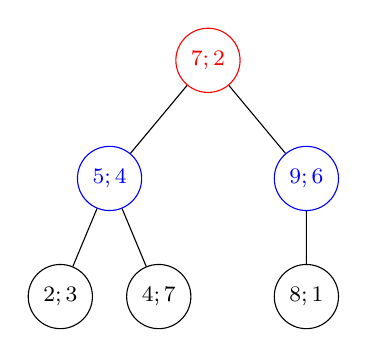
\begin{tikzpicture}[xNode/.style={circle,draw,red},
                      yNode/.style={circle,draw,blue},
                      justNode/.style={circle,draw,black},
                      level distance=1.5cm,
                      level/.style={sibling distance=2.5cm/#1},
                      font=\footnotesize]
    \node [xNode] at (0,0) {$7; 2$}
      child { node [yNode] {$5; 4$}
        child { node [justNode] {$2; 3$} }
        child { node [justNode] {$4; 7$} } }
      child { node [yNode] {$9; 6$}
        child { node [justNode] {$8; 1$} } };
  \end{tikzpicture}
  \caption{Пример kd дерева.}
  \label{ml:knn:kdtree-pic}
\end{figure}

\begin{figure}[htb]
  \centering
  \begin{tikzpicture}
    \begin{axis}[
      xlabel=$x$,
      ylabel=$y$,
      xmin=0, xmax=10,
      ymin=0, ymax=10]

      \draw [red] (axis cs:7,0)
        -- (axis cs:7,10);

      \draw [blue] (axis cs:0,4)
        -- (axis cs:7,4);

      \draw [blue] (axis cs:7,6)
        -- (axis cs:10,6);

      \addplot[
        scatter/classes={
          x={mark=square*,red},%
          y={mark=square*,blue},%
          n={mark=square*,black}
        },
        scatter,only marks,
        scatter src=explicit symbolic]
        coordinates {
          (7,2) [x]
          (5,4) [y]
          (9,6) [y]
          (2,3) [n]
          (4,7) [n]
          (8,1) [n]
        };
    \end{axis}
  \end{tikzpicture}
  \caption{Изображение kd дерева на плоскости.}
  \label{ml:knn:kdtree-2d}
\end{figure}
